\begin{figure}
  \centering
  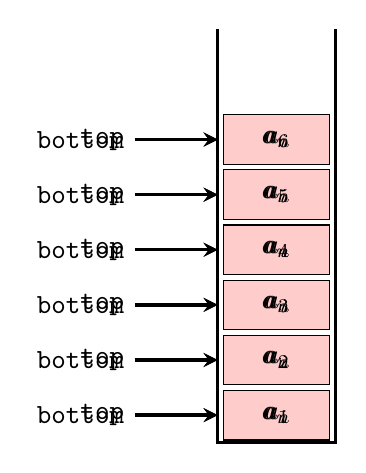
\begin{tikzpicture}
    \tikzstyle{information text}=[rounded corners,fill=blue!20,inner sep=1ex]
    \def\x{1.5}
    \def\y{0.7}
    \def\r{8}
        
    \draw[very thick] (\r,7.5*\y)--(\r,0*\y)--(\r+\x,0*\y)--(\r+\x,7.5*\y);
    
    \foreach \c in {1,2,...,6}{
      \filldraw[fill=red!40,fill opacity=0.5] (\r+0.05*\x,\c*\y-0.95*\y)rectangle(\r+0.95*\x,\c*\y-0.05*\y);
      \ifthenelse{\c=3 \OR \c=5}{
        \node [] at (\r+0.5*\x,\c*\y-0.5*\y) {$\cd$};
      }{
        \ifthenelse{\c=1 \OR \c=2}{
          \node [] at (\r+0.5*\x,\c*\y-0.5*\y) {$a_\c$};
          \ifthenelse{\c=1}{
            \draw[->,>=stealth,very thick] (\r-0.7*\x,\c*\y-0.5*\y) node[left] {\tt{bottom}}--(\r+0,\c*\y-0.5*\y);
          }{}
        }{
          \ifthenelse{4=\c }{
            \node [] at (\r+0.5*\x,\c*\y-0.5*\y) {$a_i$};
          }{
            \node [] at (\r+0.5*\x,\c*\y-0.5*\y) {$a_n$};
            \draw[->,>=stealth,very thick] (\r-0.7*\x,\c*\y-0.5*\y) node[left] {\tt{top}}--(\r+0,\c*\y-0.5*\y);
          }
        }
      }
    }
  \end{tikzpicture}
\end{figure}
